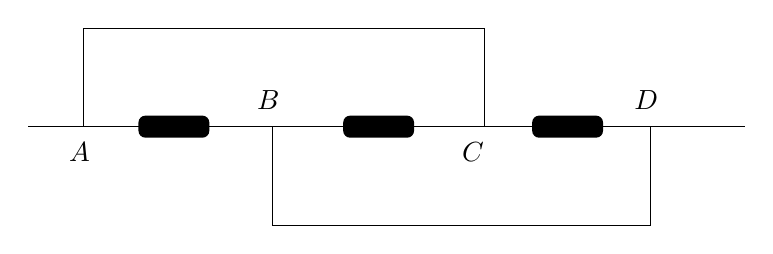
\begin{tikzpicture}
  % main horizontal line: A -- R -- B -- R -- C -- R -- D
  \draw (0.2,0) -- (9.3,0);
  % three resistor boxes (filled, rounded) on the line
  \fill[rounded corners=2.5pt] (1.6,-0.14) rectangle (2.5,0.14);
  \fill[rounded corners=2.5pt] (4.2,-0.14) rectangle (5.1,0.14);
  \fill[rounded corners=2.5pt] (6.6,-0.14) rectangle (7.5,0.14);
  % node labels
  \node[below] at (0.85,-0.08) {$A$};
  \node[above] at (3.25,0.1) {$B$};
  \node[below] at (5.85,-0.08) {$C$};
  \node[above] at (8.05,0.1) {$D$};
  % top wire: A to C
  \draw (0.9,0) -- (0.9,1.25) -- (6.0,1.25) -- (6.0,0);
  % bottom wire: B to D
  \draw (3.3,0) -- (3.3,-1.25) -- (8.1,-1.25) -- (8.1,0);
\end{tikzpicture}
